\documentclass{article}
\usepackage{graphicx}
\usepackage[margin=1.5cm]{geometry}
\usepackage{amsmath}
\usepackage{url}

\begin{document}

\title{PhET: Bending Light}
\author{Prof. Jordan C. Hanson}

\maketitle

\section{Memory Bank}

\begin{itemize}
\item \textbf{Optics:} Snell's Law states that, for an interface between two media with \textit{indices of refraction} $n_1$ and $n_2$, light leaves one medium with an angle $\theta_1$ and enters the second medium with an angle $\theta_2$ as follows:
\begin{equation}
n_1 \sin\theta_1 = n_2\sin\theta_2 \label{eq:1}
\end{equation}
\noindent The two angles are defined with respect to vertical.
\item \textbf{Optics:} Fresnel's equations give the fraction of power (in light) that is reflected ($R$) or transmitted ($T$) by an interface between media with indices of refraction $n_1$ and $n_2$:
\begin{equation}
R = \left| \frac{n_1 - n_2}{n_1 + n_2} \right|^2 \label{eq:2}
\end{equation}
\noindent Note that, to conserve power, $T = 1 - R$.
\item \textbf{Optics:} When light hits an interface at an angle, Fresnel's equations must be modified:
\begin{equation}
R = \left| \frac{n_1\cos\theta_1 - n_2\cos\theta_2}{n_1\cos\theta_1 + n_2\cos\theta_2} \right|^2 \label{eq:3}
\end{equation}
\item PhET simulation: \url{https://phet.colorado.edu/en/simulations/bending-light}
\end{itemize}

\section{Light Can Refract and Reflect}

\begin{enumerate}
\item Navigate to the PhET simuation above.  (a) Click on the introduction tab, and activate the laser by pressing the red button. Set the upper index of refraction to 1.0 and the lower index of refraction to 1.6 using the controls at the right.  (b) Using the protractor, measure the incident angle with respect to vertical, and the transmission angle with respect to vertical.  Repeat this measurement for 15 different angles between 0 and 90 degrees (with respect to vertical).  (c) Solve Snell's law for the transmission angle (Eq. \ref{eq:1}). (d) Create a 2D scatter plot in Excel, and add your prediction from Snell's law to the graph.  Do the data match the prediction?
\clearpage
\item Click on the More Tools tab below, and (a) switch the upper medium to glass and the lower to air.  (b) Using the intensity meter, determine the fraction of power reflected and trasmitted versus angle. (c) Do the data agree with Fig. \ref{fig:1} below?  We are using the $R_s$ (blue) curves. (d) At what angle do you observe total internal reflection (that is, no transmitted power)?
\end{enumerate}

\begin{figure}
\centering
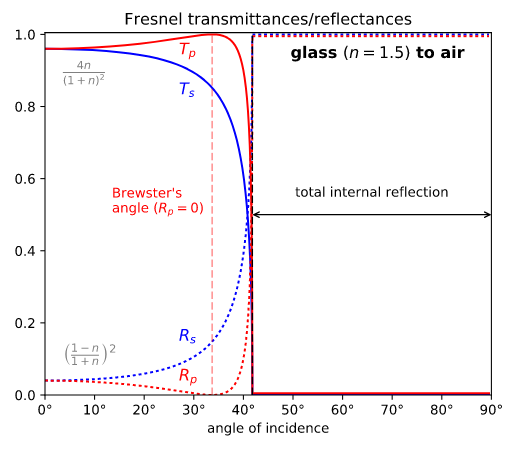
\includegraphics[width=0.5\textwidth]{figures/fresnel.png}
\caption{\label{fig:1} The Fresnel equations plotted for light moving from glass to air.}
\end{figure}

\end{document}
